\chapter{Potential Research Directions} % Main chapter title

\label{Chapter7}


We propose some potential research directions by further making use of the relationship between dependencies and our downstream structured prediction tasks (i.e., NER and semantic parsing). 
Specifically, the property that ``\textit{entities often form subtrees}'' allows us to design a joint model for joint dependency parsing and named entity recognition (Section \ref{sec:jointdepner}).
On the other hand, as we show that our dependency-based hybrid trees~\cite{jie2018dependency} not only have a good performance on English but especially on other languages where word order matters~\cite{ahmad2019difficulties}. 
The natural question for NER is: \textit{Is the linear-chain structure always the best for every language?}  
By answering this question, we attempt to build the NER system exploring different graphical models besides just linear-chain structures. 
Finally, as the dependency-based hybrid trees are flexible, we could propose a universal dependency-based hybrid tree framework for different kinds of meaning representations.



\section{Joint Dependency Parsing and Named Entity Recognition}
\label{sec:jointdepner}

Dependency grammar has gained significant attention in research field thanks to its efficiency and simplicity compared to phrase-structure parsing. 
Unlike a phrase structure, there is no phrasal node in a dependency structure; each node in a dependency structure represents a word-token in a sentence except for a root node. 
Dependencies refer to both syntactic and semantic relations between nodes. Using the dependency information can enhance the performance for some tasks like named entity recognition (NER), semantic role labeling (SRL) and semantic parsing \cite{kazama2008inducing,ling2012fine,johansson2008dependency,hacioglu2004semantic,poon2009unsupervised}.  
In dependency parsing, the basic first-order model \cite{eisner1996three} is defined by a decomposition of a tree into head-modifier dependencies. 
The syntactic relationship is represented by a directed arc between a \textit{head} word and a \textit{modifier} word. The $head$ word is considered more important in this relationship and the \textit{modifier} word is supplementing the meaning of the \textit{head} word. For example, Figure \ref{fig:dependency} shows an example of a dependency structure, which contains a dependency from the head word ``$from$'' to the modifier word ``$States$'' and this dependency infers some relationship between this two words.

\begin{figure}[h]
	\centering
	\begin{tikzpicture}[node distance=0.5mm and 0.5mm]
	\node [](root_node) at (-0.5,0) [label=below:\textit{*}]{ROOT};
	\node [](he_node) [label=below:\textit{PRP}, right=of root_node]{He};
	\node [](comes_node) [label=below:\textit{VBZ}, right=of he_node]{comes};
	\node [](from_node) [label=below:\textit{IN}, right=of comes_node]{from};
	\node [](the_node)  [label=below:\textit{DT}, right=of from_node]{the};
	\node [](united_node) [label=below:\textit{NNP}, right=of the_node]{United};
	\node [](states_node)  [label=below:\textit{NNPS}, right=of united_node]{States};
	\draw [line width=1pt, -{Stealth[length=3.5mm, open]}] (root_node) to [out=70,in=90,looseness=1.1] node [above] {} (comes_node);
	\draw [line width=1pt, -{Stealth[length=3.5mm, open]}] (comes_node) to [out=70,in=110,looseness=1.1] node [above] {} (from_node);
	\draw [line width=1pt, -{Stealth[length=3.5mm, open]}] (comes_node) to [out=120,in=50] node [above] {} (he_node);
	\draw [line width=1pt, -{Stealth[length=3.5mm, open]}] (from_node) to [out=70,in=90,looseness=1] node [above] {} (states_node);
	\draw [line width=1pt, -{Stealth[length=3.5mm, open]}] (states_node) to [out=120,in=70,looseness=1] node [above] {} (united_node);
	\draw [line width=1pt, -{Stealth[length=3.5mm, open]}] (states_node) to [out=110,in=80,looseness=1] node [above] {} (the_node);
	\draw [rounded corners] (4.4,-0.2) rectangle (7.3,0.2);
	\end{tikzpicture}
	\caption{An example dependency structure given a sentence and its POS tags. ``$United$ $States$'' is a \textit{location} entity.}
	\label{fig:dependency}
\end{figure}




However, this kind of dependency only captures the relationship between individual words while ignoring the integrity of multiple words. As in the example shown in Figure \ref{fig:dependency}, ``$United$ $States$'' is an entity with the type of \textit{location}. 
The words ``$United$ $States$'' (the rounded rectangle in Figure \ref{fig:dependency}) should be considered a group in the dependency structure. 
Thus we do not need to parse the whole entity into single words, such that we can capture the relationship between $from$ and $United$ $States$ instead of $from$ and $States$. One of the advantages of doing this is helping us to extract the predicate information like ``comes\_from(\textit{He}, /ENTITY/\textit{United States})'' in this example. 
This kind of structure with embedded entity information will further facilitate the other applications like SRL and semantic parsing. To the best of our knowledge, this is the first work focusing on the task of joint dependency parsing and named entity recognition. 
% draw a rectangle to the figure

We would like to present a new joint model for efficient dependency parsing and named entity recognition, which is a feature-based CRF model over hybrid-tree structure \cite{lu2008generative,klein2004parsing}. 
%We demonstrate our model can jointly generate consistent named entities and dependency structures. 
%We evaluate our model on the SemEval 2010 task 1 dataset which is a subset of OntoNotes 2.0 release. In general, we make the following contributions:
%\begin{itemize}
%	\item We propose a novel model that is able to jointly capture dependencies and named entity information.
%	\item We demonstrate that our model can achieve a competitive performance compared to other models doing the individual task.
%\end{itemize}
  
%\url{http://statnlp.org/research/dp/}.
\subsection{Eisner's First-order Parser}

In our joint model, we need to maintain the original dependency structure which is the first-order model introduced by \cite{eisner2000bilexical}. 
The first-order dynamic programming structure and derivation are shown in Figure \ref{fig:derivation}. 
We summarize the dynamic programming derivation here and later we can understand our joint model clearly. 
\begin{figure}[h!]
	\centering
	\begin{subfigure}{1\linewidth}
		\centering
		\begin{tikzpicture}
		\node [scale = 1](a) at (-0.6,0.5) {(a)};
		\draw [line width = 1pt] (1.5,0) node [below=0.05cm] {$e$} -- (-0.2,0) node [below] {$h$} -- (-0.2,1) -- cycle;
		\draw [->,line width = 1pt] (1.6,0.5) -- (2.2,0.5);
		\draw [line width = 1pt] (3.9,0) node [below=0.05cm] {$m$} -- (2.4,0) node [below] {$h$} -- (2.4,1)-- (3.9,0.7) -- cycle;
		\draw [line width=1pt, -{Stealth[length=4mm, open]}] (2.4,0) to [out=70,in=120] node [above] {} (3.9,0);
		\node [scale = 1.5](equals) at (4.4,0.5) {+};
		\draw [line width = 1pt] (6.2,0) node [below=0.05cm] {$e$} -- (4.9,0) node [below=0.05cm] {$m$} -- (4.9,0.7) -- cycle;
		\end{tikzpicture}
%		\caption{Derivation of a complete span.} 
%		\label{fig:complete}
	\end{subfigure}
	\begin{subfigure}{1\linewidth}
		\centering
		\begin{tikzpicture}
		\node [scale = 1](a) at (-0.6,0.5) {(b)};
		\draw [line width = 1pt] (1.5,0) node [below=0.05cm] {$m$} -- (-0.2,0) node [below] {$h$} -- (-0.2,1) -- (1.5,0.7) -- cycle;
		\draw [line width=1pt, -{Stealth[length=4mm, open]}] (-0.2,0) to [out=70,in=120] node [above] {} (1.5,0);
		\draw [->,line width = 1pt] (1.7,0.5) -- (2.3,0.5);
		\draw [line width = 1pt] (4.1,0) node [below=0.05cm] {$e$} -- (2.6,0) node [below] {$h$} -- (2.6,1)-- cycle;
		\node [scale = 1.5](equals) at (4.4,0.5) {+};
		\draw [line width = 1pt] (6.2,0) node [below=0.05cm] {$m$} -- (4.9,0) node [below] {$e+1$} -- (6.2,0.7) -- cycle;
		\end{tikzpicture}
%	\caption{Derivation of an incomplete span.} 
%	\label{fig:incomplete} 
\end{subfigure}
	\caption{The dynamic-programing structures and derivation of the first-order model. (a) complete span, (b) incomplete span. Only right-direction derivation is shown due to space limit. }
	\label{fig:derivation}
\end{figure}

There are two basic data structures in this dynamic-programming derivation: one is called \textit{complete} span and another one is called \textit{incomplete} span. 
A complete span, referred to Figure \ref{fig:derivation}(a), consist of a head word $h$ and a end word $e$. 
In this span, only the head word has no parent, all the other words in the span are already attached to a parent word.  
For the incomplete span, referred to Figure \ref{fig:derivation}(b), there is still a head word $h$ but the word $m$ at the other end is not complete yet. 
There is also an explicit dependency from a head word $h$ to a modifier word $m$ indicated on the span. 

Followed the notation from this work \cite{koo2010efficient}, a complete span is denoted as $C_{h,e}$ and an incomplete span is denoted as $I_{h,m}$. As shown in Figure \ref{fig:derivation}, a complete span can be decomposed to the combination of an incomplete span and a complete span. The index $m$ in Figure \ref{fig:derivation}(a) is the split point for this decomposition. An incomplete span can be decomposed to two complete spans where there is also a free index $e$ in Figure \ref{fig:derivation}(b). 
To parse a sentence into a dependency structure, we are essentially finding a construction process that can form the complete span from the first word (root) to the last word. 
The dependency structure can then be extracted from all the incomplete spans where contains an arc from the $h$ to $m$.
Using a chart-parsing algorithm like CKY can help us efficiently parse the sentence into this structure. 



\subsection{Joint Dependency and Named Entity Model}
In order to apply the dynamic programming technique in our joint model, we used similar derivation in the first-order parsing model. 
Figure \ref{fig:ourmodelderivation} shows the dynamic programming derivation of our joint model. The intuition behind is that each span in the derivation can be represented as a type, which can be \textit{person}, \textit{organization}, \textit{GPE}, \textit{MISC}. 
Besides entity type, we introduced two more types that can facilitate our model later. A type \textbf{\textit{E}} which indicates there is at least one entity inside this span and a type \textbf{\textit{N}} which indicates there is no entity inside this span. We use a label \textbf{\textit{T}} to include all this three types: \textit{E}, \textit{N} and entity types. 

In addition to complete spans and incomplete spans in the first-order model, we augmented the span type with \textit{general} spans and \textit{typed} spans. 
For a general span, there is no type information attached with it and but it has a symbol that can record its parent's type as in Figure \ref{fig:ourmodelderivation}(a) and Figure \ref{fig:ourmodelderivation}(b) the children have a symbol to store the type of their parent. 
The general spans can be decomposed to a typed span with a specific entity type as shown in Figure \ref{fig:ourmodelderivation}(a) and Figure \ref{fig:ourmodelderivation}(b). The type \textit{T}' attached with the child and the \textit{L} in the parent's symbol may not be the same since the child span might have other types that are not required to be same as the larger span. 
For example, a span (\textit{h},\textit{m}) with a type \textit{E} can have a smaller span inside that is attached with a type \textit{person}. 

Following the above example, we should define some rules that what types that smaller spans can have according to the type of their grandparents. Table \ref{tab:typerule} shows the rule that can be applied in our model. Since we can only look at the relationship between children and parent in our derivation, we are able to capture the exact relationship between a larger typed span and the two smaller typed spans which compose the larger span. 
%%%%%%%
%%%%%%%
%%%% think about how to explain this, use a figure
\begin{table}[h]
	\centering
	\begin{tabular}{cc}
		\toprule
		parent type & child type \\   \midrule
		\textit{E}' & \textit{E}, \textit{N}, \textit{person}\\ 
		\textit{N}' & \textit{N}\\
		\textit{person}' & \textit{person}\\ 
		\bottomrule
	\end{tabular}
	\caption{Derivation rule for the typed spans. Derivation for other entity types like GPE are same as \textit{person}. They are not shown in the table due to space limit.}
	\label{tab:typerule}
\end{table}
Since type \textit{E} means at least one entity inside this span, so the child type can be either \textit{E}, \textit{N} or \textit{person}. If the parent type is already \textit{N} or \textit{person}, then we define that the child type must be same as the parent type since there is also no nested entities in our dataset. 

To parse a sentence, our model tries to find an optimal construction of the sentence over all the possible hybrid-tree structure built by the derivation. 
This can be done similarly as the first-order parsing by the chart-parsing technique. 
The decomposition process (Figure \ref{fig:ourmodelderivation}(a) and \ref{fig:ourmodelderivation}(b)) of the typed span is same as first-order parsing since the entity type \textit{T} is not the free parameters like the third free index (the split point).
Since each derivation is at most defined by two fixed indices and an entity type, this parsing algorithm will need $\mathcal{O}(n^{2}|T|)$ space. The complexity of our parsing algorithm is still $\mathcal{O}(n^{3}|T|)$, where $n$ is the length of a sentence. 
\begin{figure}[h]
	\centering
	\begin{subfigure}{0.45\linewidth}
		\centering
		\begin{tikzpicture}
		\node [scale = 1](a) at (-0.6,0.5) {(a)};
		\draw [line width = 1pt] (1.5,0) node [below=0.05cm] {$e$} -- (-0.2,0) node [below] {$h$} -- (-0.2,1) -- cycle;
		\node [](type) at (0.4, 0.3) {\textit{T}};
		\draw [->,line width = 1pt] (1.6,0.5) -- (2.2,0.5);
		\draw [line width = 1pt] (3.9,0) node [below=0.05cm] {$m$} -- (2.4,0) node [below] {$h$} -- (2.4,1)-- (3.9,0.7) -- cycle;
		\node [](pa_type1) at (3.1, 0.57) {\textit{T}'};
		\draw [line width=1pt, -{Stealth[length=4mm, open]}] (2.4,0) to [out=70,in=120] node [above] {} (3.9,0);
		\node [scale = 1.5](equals) at (4.4,0.5) {+};
		\draw [line width = 1pt] (6.2,0) node [below=0.05cm] {$e$} -- (4.9,0) node [below=0.05cm] {$m$} -- (4.9,0.7) -- cycle;
		\node [](pa_type2) at (5.25, 0.2) {\textit{T}'};
		\end{tikzpicture}
	\label{fig:modelcomplete} 
\end{subfigure}
	\begin{subfigure}{0.45\linewidth}
		\centering
		\begin{tikzpicture}
		\node [scale = 1](a) at (-0.6,0.5) {(b)};
		\draw [line width = 1pt] (1.5,0) node [below=0.05cm] {$m$} -- (-0.2,0) node [below] {$h$} -- (-0.2,1) -- (1.5,0.7) -- cycle;
		\node [](type) at (0.6, 0.65) {\textit{T}};
		\draw [line width=1pt, -{Stealth[length=4mm, open]}] (-0.2,0) to [out=70,in=120] node [above] {} (1.5,0);
		\draw [->,line width = 1pt] (1.7,0.5) -- (2.3,0.5);
		\draw [line width = 1pt] (4.1,0) node [below=0.05cm] {$e$} -- (2.6,0) node [below] {$h$} -- (2.6,1)-- cycle;
		\node [](pa_type1) at (3.1, 0.3) {\textit{T}'};
		\node [scale = 1.5](equals) at (4.4,0.5) {+};
		\draw [line width = 1pt] (6.2,0) node [below=0.05cm] {$m$} -- (4.9,0) node [below] {$e+1$} -- (6.2,0.7) -- cycle;
		\node [](pa_type2) at (5.7, 0.2) {\textit{T}'};
		\end{tikzpicture}
	\label{fig:modelincomplete} 
\end{subfigure}
	\begin{subfigure}{0.45\linewidth}
		\centering
		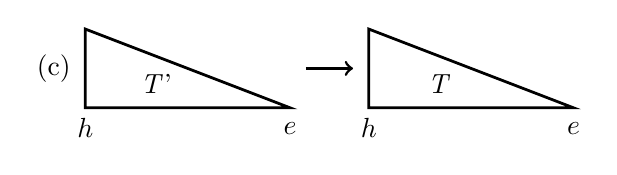
\begin{tikzpicture}
		\node [scale = 1](a) at (-0.6,0.5) {(c)};
		\draw [line width = 1pt] (2.4,0) node [below=0.05cm] {$e$} -- (-0.2,0) node [below] {$h$} -- (-0.2,1) -- cycle;
		\node [](pa_type1) at (0.7, 0.3) {\textit{T}'};
		\draw [->,line width = 1pt] (2.6,0.5) -- (3.2,0.5);
		\draw [line width = 1pt] (6.0,0) node [below=0.05cm] {$e$} -- (3.4,0) node [below] {$h$} -- (3.4,1)-- cycle;
		\node [](type) at (4.3, 0.3) {\textit{T}};
		\end{tikzpicture}
	\label{fig:generalcomplete}
\end{subfigure} 
	\begin{subfigure}{0.45\linewidth}
		\centering
		\begin{tikzpicture}
		\node [scale = 1](a) at (-0.4,0.5) {(d)};
		\draw [line width = 1pt] (2.6,0) node [below=0.05cm] {$m$} -- (0,0) node [below] {$h$} -- (0,1.3) -- (2.6,0.8) -- cycle;
		\node [](pa_type1) at (0.9, 0.7) {\textit{T}'};
		\draw [line width=1pt, -{Stealth[length=4mm, open]}] (0,0) to [out=50,in=140] node [above] {} (2.6,0);
		\draw [->,line width = 1pt] (2.8,0.5) -- (3.4,0.5);
		\draw [line width = 1pt] (6.1,0) node [below=0.05cm] {$m$} -- (3.6,0) node [below] {$h $} -- (3.6,1.2)-- (6.1,0.8) -- cycle;
		\draw [line width=1pt, -{Stealth[length=4mm, open]}] (3.6,0) to [out=50,in=140] node [above] {} (6.1,0);
		\node [](type) at (4.5, 0.7) {\textit{T}};
		\end{tikzpicture}
	\label{fig:generalincomplete} 
\end{subfigure}
	\caption{The dynamic-programming structures and derivation of our joint dependency parsing and named entity recognition model. Typed spans are decomposed to general spans and general spans are decomposed to typed spans.}.
	\label{fig:ourmodelderivation}
\end{figure}


By jointly parsing the entity and dependency together, they can interact and help each other in the joint model. 
We found that most of the named entities in our dataset have an outmost dependency that headed by either the beginning or the end of an entity. 
Inspired by this structure, we can then extract the joint features in this kind of span and as well as their entity features and dependency features. 
For example, the dependency structure of an organization entity \textit{National University of Singapore} is shown in Figure \ref{fig:jointsmallexample}.
\begin{figure}
	\centering
	\begin{tikzpicture}[node distance=4mm and 5mm]
	\node [](a_node) []{National};
	\node [](b_node) [right=of a_node] {University};
	\node [](c_node) [right=of b_node] {of};
	\node [](d_node) [right=of c_node]{Singapore};
	\node [](at_node) [label=below:\textit{B-org},below=of a_node,yshift=5mm]{\textit{NNP}};
	\node [](bt_node) [label=below:\textit{I-org}, below=of b_node,yshift=5mm] {\textit{NNP}};
	\node [](ct_node) [label=below:\textit{I-org},below=of c_node,yshift=5mm] {\textit{IN}};
	\node [](dt_node) [label=below:\textit{I-org},below=of d_node,yshift=5mm]{\textit{NNP}};
	\draw [line width=1pt, -{Stealth[length=3.5mm, open]}] (d_node) to [out=120,in=60, looseness=0.5] node [above] {} (a_node);
	\draw [line width=1pt, -{Stealth[length=3.5mm, open]}] (d_node) to [out=120,in=60, looseness=0.5] node [above] {} (b_node);
	\draw [line width=1pt, -{Stealth[length=3.5mm, open]}] (d_node) to [out=120,in=60, looseness=0.5] node [above] {} (c_node);
	\end{tikzpicture}
	\caption{An organization entity in dependency structure.}
	\label{fig:jointsmallexample}
\end{figure}
With the derivation in Figure \ref{fig:ourmodelderivation}, the above entity forms an incomplete span from \textit{National} to \textit{Singapore}. 
This typed span is headed by \textit{Singapore} and ended at \textit{National}. 
We can then extract the whole entity features with the help of dependency information.
In a similar way, the entity information can help identify the head or modifier to find the best dependency structure. 





%\subsection{Special Case}
%\label{sec:sepcialcase}
%Following the derivation of our model, each entity with more than one word is correlated to an incomplete span in our parse tree. 
%However, not all the entities follow incomplete span structure. 
%This section will point out this case and how we try to solve them. 
%The problem is that an entity is governed by two or more spans and our model will classify each span is an unique entity, which results in one entity would be split into two span without the entity label by our model. 
%We call this case ``invalid'' span. 
%For instance, Figure \ref{fig:specialexamples} shows two example structure of this case from the training data. 
%\begin{figure*}
%	\centering
%	\begin{subfigure}{0.45\linewidth}
%		\centering
%		\begin{tikzpicture}[node distance=2.9mm and 2.9mm]
%		\node [scale = 1](a_start) [] {(a)};
%		\node [](a_node) [ right=0.5mm of a_start] {Source};
%		\node [](b_node) [right=of a_node] {$\cdots$} ;
%		\node [](c_node) [right=of b_node] {Telerate};
%		\node [](d_node) [ right=of c_node] {Systems};
%		\node [](e_node) [right=of d_node] {Inc};
%		
%		\node [](at_node) [label=below:\textit{O},below=of a_node,yshift=5mm]{\textit{NNP}};
%		\node [](bt_node) [label=below:$\cdots$ ,below=of b_node,yshift=2.5mm] {$\cdots$};
%		\node [](ct_node) [label=below:\textit{B-org},below=of c_node,yshift=5mm] {\textit{IN}};
%		\node [](dt_node) [label=below:\textit{I-org},below=of d_node,yshift=5mm]{\textit{NNP}};
%		\node [](et_node) [label=below:\textit{I-org},below=of e_node,yshift=5mm]{\textit{NNP}};
%		
%		\draw [line width=1pt, -{Stealth[length=3.5mm, open]}] (a_node) to [out=60,in=110, looseness=0.6] node [above] {} (d_node);
%		\draw [line width=1pt, -{Stealth[length=3.5mm, open]}] (d_node) to [out=120,in=60, looseness=0.6] node [above] {} (c_node);
%		\draw [line width=1pt, -{Stealth[length=3.5mm, open]}] (d_node) to [out=60,in=120, looseness=0.6] node [above] {} (e_node);
%		\end{tikzpicture}
%	\label{fig:special1} 
%\end{subfigure}
%		\begin{subfigure}{0.45\linewidth}
%			\centering
%		\begin{tikzpicture}[node distance=3mm and 3mm]
%		\node [scale = 1](b_start) [] {(b)};
%		\node [](a_node_1) [ right=of b_start] {Peoples};
%		\node [](b_node_1) [right=of a_node_1] {Drug} ;
%		\node [](c_node_1) [right=of b_node_1] {Store};
%		\node [](d_node_1) [right=of c_node_1] {Inc.};
%		\node [](e_node_1) [right=of d_node_1] {unit};
%		
%		\node [](at_node) [label=below:\textit{B-org},below=of a_node_1,yshift=5mm]{\textit{NNP}};
%		\node [](bt_node) [label=below:\textit{I-org} ,below=of b_node_1,yshift=5mm] {\textit{NNP}};
%		\node [](ct_node) [label=below:\textit{I-org},below=of c_node_1,yshift=5mm] {\textit{IN}};
%		\node [](dt_node) [label=below:\textit{I-org},below=of d_node_1,yshift=5mm]{\textit{NNP}};
%		\node [](et_node) [label=below:\textit{O},below=of e_node_1,yshift=5mm]{\textit{NNP}};
%		
%		\draw [line width=1pt, -{Stealth[length=3.5mm, open]}] (e_node_1) to [out=120,in=60, looseness=0.6] node [above] {} (a_node_1);
%		\draw [line width=1pt, -{Stealth[length=3.5mm, open]}] (e_node_1) to [out=120,in=60, looseness=0.6] node [above] {} (b_node_1);
%		\draw [line width=1pt, -{Stealth[length=3.5mm, open]}] (e_node_1) to [out=120,in=60, looseness=0.6] node [above] {} (c_node_1);
%		\draw [line width=1pt, -{Stealth[length=3.5mm, open]}] (e_node_1) to [out=120,in=60, looseness=0.6] node [above] {} (d_node_1);
%		\end{tikzpicture}
%\label{fig:special2} 
%\end{subfigure}
%	\caption{Two example of the special case from training data. The entity in (a) is split into two spans and the entity in (b) is split into four spans in our model. }
%	\label{fig:specialexamples}
%\end{figure*}
%
%As shown in Figure \ref{fig:special1}, the organization entity \textit{Telerate Systems Inc} is headed by the word inside instead of one of its boundary words. Thus this entity will be split into two spans and both of them will not be recognized as an entities when constructing the structure in our model. Similar to the second case in Figure \ref{fig:special2}, the entity in dependency structure is headed by a word \textit{unit} outside the entity. In this case, all the words of will be split into a span containing only themselves rather than form an entity span for \textit{Peoples Drug Store Inc.} 
%We do not find too many entities are forming this dependency structure in our training as shown in the experiment section. Moreover, we think a more consistent dependency structure should be headed by a boundary word as in Figure \ref{fig:jointsmallexample}. Although there are some entities are in this form which we called they are inconsistent with their dependencies. We called this kind of dependency span ``invalid'' span and found a method to solve this problem. 
%
%Since our dataset does not contain any nested named entities, we revise the model that make all the spans whose words are contained by the entity become labeled span. So that in our parsing structure of the example in Figure \ref{fig:special1}, then both of the span \textit{Telerate Systems} and \textit{Systems Inc} are labeled as organization entity. 
%We combined the entities that are near each other and have the same entity type to a single entity in a sentence. 
%Using this approach may result in another problem that not all the adjacent entities with the same type can be combined into one entity. 
%However, we found that the adjacent entities with the same entity barely appear in our data. Table \ref{tab:adjacententities} shows the number of these adjacent entities in training and testing data. This case happens only four times in training data and 2 times in testing data. Thus we ignore this kind of case and combine them into one entity in our testing result. 
%
%\begin{table}[h]
%	\centering
%	\begin{tabular}{c|cc}
%		& \multicolumn{2}{c}{\#Adjacent entities(\textit{B-E}...\textit{I-E})(\textit{B-E}} \\
%		entity & Training+Dev & Testing\\   \hline
%		\textit{person} & 0 & 0 \\
%		\textit{GPE} & 3(0.2\%) & 1(0.3\%) \\
%		\textit{organization} & 1(0.08\%) & 1(0.3\%) \\
%	\end{tabular}
%	\caption{Dataset Statistics. The number of cases that two same entities are adjacent in our dataset. }
%	\label{tab:adjacententities}
%\end{table}
%
%Our model can still handle this problem if there are nested entities in the data. If there is an entity that is split into multiple spans by the dependency structure, we split the entity into multiple entities for training. For example, the entity type for \textit{Peoples Drug Store Inc.} in Figure \ref{fig:special2} will then become \textit{B-org B-org B-org B-org} since the dependency structure will split them into four spans with only a single word.  Finally, as the statistics shown above, the adjacent entities with same type will be combined into one entity. 


\subsection{Log-Linear Modeling}
Conditional random fields (CRFs)\cite{lafferty2001conditional} have been widely used in natural language processing problems like part-of-speech tagging, named entity recognition \cite{mccallum2003early} and semantic role labeling \cite{cohn2005semantic}. 
In this work, we also defined a discriminative log-linear model over the dynamic programming derivation. 

To be more specific, the probability of predicting a possible output $\vec{y}$ (a dependency tree structure with entity information in each span) given an input sentence $\vec{x}$ is given as:
\begin{equation}
p(\vec{y}|\vec{x}) = \frac{\exp(\vec{\vec{w}^{T}\vec{f}(\vec{x},\vec{y}) })}{\sum_{\vec{y}^{'}}\exp(\vec{\vec{w}^{T}\vec{f}(\vec{x},\vec{y}^{'}) })}
\end{equation}

where $\vec{f}(\vec{x},\vec{y})$ is the feature vector defined on the sentence $\vec{x}$ and the tree structure $\vec{y}$. The best tree structure should satisfy that $\vec{y}^{*} = \argmax_{\vec{y}}p(\vec{y}|\vec{x})$. 

We aim to minimize the negative joint log-likelihood with $\textit{L}_{2}$ regularization for our dataset, which defines the objective function as:
\begin{equation}
\begin{split}
\mathcal{L}(\vec{w}) = \sum_{i}\log\sum_{\vec{y}^{'}}\exp(\vec{w}^{T}\vec{f}(\vec{x}_{i},\vec{y}^{'})) - \sum_{i}\vec{w}^{T}\vec{f}(\vec{x}_{i},\vec{y}_{i}) + \lambda \vec{w}^{T}\vec{w}
\end{split}
\end{equation} 
where $(\vec{x}_{i},\vec{y}_{i})$ is the $i$-th training instance and $\lambda$ is the $L_{2}$ regularization parameter which is set to $0.7$ in our experiments. The partial derivative of $\mathcal{L}$ with respect to each parameter $w_{k}$ is:
\begin{equation}
\begin{split}
\frac{\partial\mathcal{L}}{\partial w_{k}}  = \mathbf{E}_{p(\vec{y}^{'}|\vec{x}_{i})} \left [f_{k}(\vec{x}_{i}, \vec{y}^{'})    \right ] - \sum_{i} f_{k}(\vec{x}_{i}, \vec{y}_{i}) + 2\lambda w_{k}
\end{split}
\end{equation}
The convexity and differentiability of objective function guarantees convergence to the global optimum, and using inside-outside algorithm can efficiently compute the above gradient. There are numbers of techniques can be used for optimizing objective function. We used L-BFGS \cite{byrd1995limited} as our optimization method.

%\subsection{Features}
%For the named entity features, we applied the similar feature set from \cite{finkel2009nested}.
%The features we used are defined over the span structures as shown in our derivation of Figure \ref{fig:ourmodelderivation}. We can extract the complete entities features with the benefits of our model. The model can directly obtain the information of an entity if the span is a labeled span with entity type integrated. We applied some of the entity features from \cite{lu2015joint}. Specifically, the following features are included in our experiments: 
%\begin{itemize}
%	\item Word $n$-grams (and POS $n$-grams) that contain the current word, for $n=2,3,4$.
%	\item Boundary words (and POS tags) of the entity.
%	\item All the words (and POS tags) in the entity span.
%	\item Entity type of current span
%	\item Head or modifier word (and POS tags) with the current labeled-incomplete span
%	\item The head and modifier words (and POS tags) pair of the current labeled-incomplete span 
%\end{itemize}
%In addition to entity features, we maintained the dependency structure with the form of general span. Thus our model can extract the original dependency features which are exactly same as previous work \cite{mcdonald2005online}. Furthermore, all dependency features are conjoined with the direction of span as well as the distance between leftmost and rightmost words being attached. 
%Note that all features used in our model are the indicator functions defined on spans. But for entity features, they are also associated with their corresponding entity type.

\subsection{Preliminary Experiments}
We conduct our experiments on two datasets, one is LDC2011T01 SemEval-2010 Task 1 OntoNotes English corpus \footnote{https://catalog.ldc.upenn.edu/LDC2011T01}, which is the only one we can find has both the annotated dependency and named entity information. 
The other one is the broadcast news from LDC2013T19 OntoNotes Release 5.0 \footnote{https://catalog.ldc.upenn.edu/LDC2013T19}. Following the work on named entity recognition \cite{finkel2009joint}, we use the following 6 types of documents: ABC, CNN, MNB, NBC, PRI and VOA. 
However, there is no dependency annotation in OntoNotes 5.0 dataset. 
We applied the LTH\footnote{http://nlp.cs.lth.se/software/treebank\_converter/} converter \cite{johansson2007a} to convert the constituent parse tree to dependency structure \footnote{There are some tags (e.g. META, EDITED) from OntoNotes treebank do not appeared in the penn treebank. We removed those sentences that cannot be converted. Furthermore, we also abandon the sentences with non-projective dependency after conversion.}. 



\subsection{Dataset}
This English corpus contains both the dependency relationships and named entities information, as well as the POS tag. In general, we consider the following three entity types in the dataset: \textsc{person}, \textsc{organization}, \textsc{GPE} (geo-political entity, such as a city or a country). 
There are total 3,358 sentences for training, 684 sentences in development set and 1,058 sentences for testing. 
Since we only focus on the projective dependency parsing, the sentences with non-projective dependency are eliminated in our dataset. 

\begin{table}[h]
	\centering
	\begin{tabular}{ccccc}
		\toprule
		& \multicolumn{2}{c}{Training+Dev} & \multicolumn{2}{c}{Testing}\\ 
		& invalid & \#entity  &  invalid & \#entity  \\
		\midrule
		\textsc{per} & 18 & 1,457 & 4   & 346\\ 
		\textsc{gpe} & 41   & 1,356 & 8  & 380\\ 
		\textsc{org} & 254  & 1,199 & 69  & 382\\ 
		\#total & 313  & 4,012 & 91& 1,108\\ 
		\bottomrule
	\end{tabular}
	\caption{Dataset Statistics. The total number of entities and the number of ``invalid'' entities in training and testing data. ``Invalid`` entities are the special case describe in Section \ref{sec:sepcialcase}.}
	\label{tab:jointstatistics}
\end{table}
Table \ref{tab:jointstatistics} shows the statistics of our dataset. For ``invalid'', the entity itself cannot form a continuous subtree.
We have a total of 4,012 entities in our training and development data and 1,108 entities in testing data. 
It is obvious to see that there are few invalid entities for \textsc{person} and \textsc{gpe}. 
%Although the \textsc{organization} entity is more likely to encounter the special case in dependency structure, we can fix this problem using the trick introduced in Section \ref{sec:sepcialcase}. 

\subsection{Results}

Table \ref{tab:jointnerresult} shows the NER performance of our joint model compared to linear-chain CRF model on the SemEval 2010 dataset. 
At the moment, the results of the joint model do not surpass the performance of the linear-chain CRF model. 
Such a result gives us some guidance to further improve our model as our joint model loses some information regarding the label transition. 
\begin{table*}[h!]
	\centering
	\begin{tabular}{ccccccc}
		\toprule
		& \multicolumn{3}{c}{Just NER}  & \multicolumn{3}{c}{Our Joint Model}\\
		& Precision&Recall&F-measure & Precision&Recalll&F-measure \\ 
		\midrule
		\textsc{person}& 79.08\% & 79.77\%  & 79.42\%& 79.55\%  & 80.92\%  & 80.23\% \\
		\textsc{GPE} & 78.77\% & 87.89\% & 83.08\%  & 73.72\%  & 87.11\%  & 79.86\% \\ 
		\textsc{organization} & 67.53\%   & 54.45\% & 60.29\%  &59.01\% & 43.72\% & 50.23\% \\
		\textsc{MISC} & 80.11\%   & 63.32\% & 70.73\%   & 75.79\% & 67.69\% & 71.51\%  \\
		Overall & \textbf{76.78\%}   & \textbf{70.75\%} & \textbf{73.65\%}  & 72.87\% & 69.48\% & 71.13\% \\
		\bottomrule
	\end{tabular}
	\caption{Named Entity Recognition Results on SemEval 2010 dataset with both dependency and named entity information annotated. }
	\label{tab:jointnerresult}
\end{table*}




\section{Dependency as Graphical Models for NER}
As different languages have different word order~\cite{ahmad2019difficulties}, we believe that the classic linear-chain structures might not always be the perfect solution for NER in every language. 
To this end, we propose to use the universal dependencies as guidance for building the graphical model. 
Our goal is to build a graphical model that follows the universal dependency trees but enjoys the linear-time complexity as in the linear-chain CRF model. 




\section{Universal Hybrid Tree Framework for Semantic Parsing}

As mentioned in Chapter \ref{Chapter2}, we have many types of meaning representations such as lambda-calculus expression, FunQL, AMR, and SQL. 
However, researchers proposed different models for different types of meaning representations. 
We argue that it is not practical to have many different models in this scenario. 
In order to achieve a semantic parser that can easily adapt to different meaning representation, we propose a prototype of a dependency-based hybrid tree framework.
As the hybrid tree framework only requires hybrid tree grammar for us to build a general parser. 
We propose a series of general hybrid tree grammar that potentially apply to all types of meaning representation.

%\subsection{General Hybrid Tree Grammar}